\documentclass[11pt,twocolumn]{article}
\usepackage{lmodern,setspace,amsmath,amssymb,amsfonts,amsthm,graphicx,multicol,grffile,float}
\usepackage[a4paper, top=0.9in, bottom=1.05in, left=1.05in, right=1.05in]{geometry}
\usepackage[digitsep={ }]{siunitx}
\usepackage[polish]{babel}
\usepackage[utf8]{inputenc}
\usepackage[T1]{fontenc}
\title{Algorytmy i struktury danych - Sortowanie}
\author{Dariusz Max Adamski}
\date{}

\begin{document}

\maketitle



\section*{Wstęp}

W tym sprawozdaniu porównywana będzie efektywność różnych algorytmów sortujących, w odniesieniu do ich złożoności obliczeniowej, zużycia pamięci i czasu wykonywania. Brane pod uwagę będą także przypadki krańcowe, czyli dane wejściowe, dla których algorytm może mieć zdecydowanie dłuższy czas wykonywania, niż dla ciągu złożonego z liczb losowych.



\section*{Metodologia}

Pomiary były wykonywane na tablicach o wielkości od $1\ 000$ elementów do $15\ 000$ elementów, z krokiem $1\ 000$ elementów (15 punktów pomiarowych). Wkonane zostały także pomiary na tablicach o wielkości od $50\ 000$ elementów do $1\ 000\ 000$ elementów, z krokiem $50\ 000$ elementów (20 punktów pomiarowych). Przypadki w których czas wykonywania był kwadratowy nie były testowane na tablicach większych od $15\ 000$ elementów. Jako punkt odniesienia, na wykresach zostały także umieszczone czasy dla algorytmu sortowania z biblioteki standardowej języka C++ (oznaczony jako ,,C++ sort''). Losowe liczby były generowane w przedziale $[1,10\ 000]$, z równomiernym rozkładem prawdopodobieństwa. Optymalizacja kompilatora została wyłączona flagą ,,-O0''. Czas wykonywania był mierzony w nanosekundach.



\section{Algorytmy}

\noindent {\bf Bubble sort BS} to algorytm sortujący w miejscu (nie zużywa dodatkowej pamięci), o złożoności obliczeniowej $O(n^2)$ w najlepszym, średnim i najgorszym przypadku.

\noindent {\bf Counting sort CS} to algorytm o złożoności obliczeniowej $O(n+k)$ w każdym przypadku. Nie sortuje w miejscu.

\noindent {\bf Quicksort QS} jest algorytmem o złożoności obliczeniowej $O(n \log n)$ w najlepszym i średnim przypadku, a w najgorszym przepadku $O(n^2)$. Może sortować w miejscu.

\noindent {\bf Merge sort MS} jest algorytmem o złożoności obliczeniowej $O(n \log n)$ w najlepszym, średnim i najgorszym przypadku. Nie sortuje w miejscu.

\noindent {\bf Heap sort HS} jest algorytmem sortującym w miejscu, o złożoności obliczeniowej $O(n \log n)$ w najgorszym, średnim i najlepszym przypadku.

\noindent {\bf Shell sort ShS} jest algorytmem sortującym w miejscu, o złożoności obliczeniowej (dla użytej implementacji) $O(n^{1.25})$ w najgorszym, średnim i najlepszym przypadku.


\section{Pomiary BS HS CS ShS}

Pierwszymi porównywanymi algorytmami będą bubble sort BS, heap sort HS, counting sort CS oraz Shell sort ShS.



\subsection{Dane losowe małe}

\begin{figure}[h]
	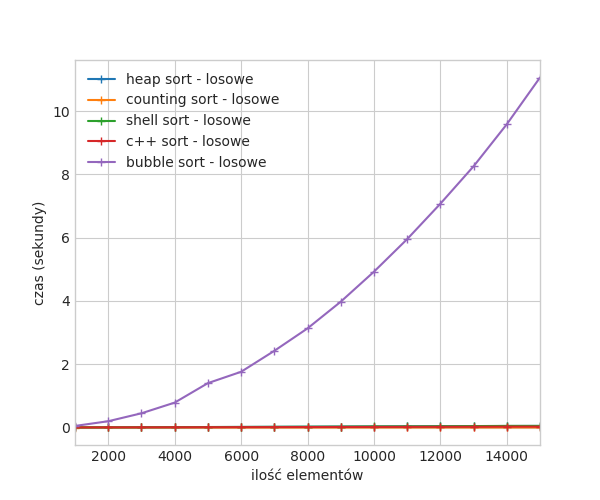
\includegraphics[width=\linewidth]{plots/los_bub_small.png}
	\caption{Czas sortowania danych losowych (małe dane) \label{losowe_male}}
\end{figure}

\begin{figure}[h]
	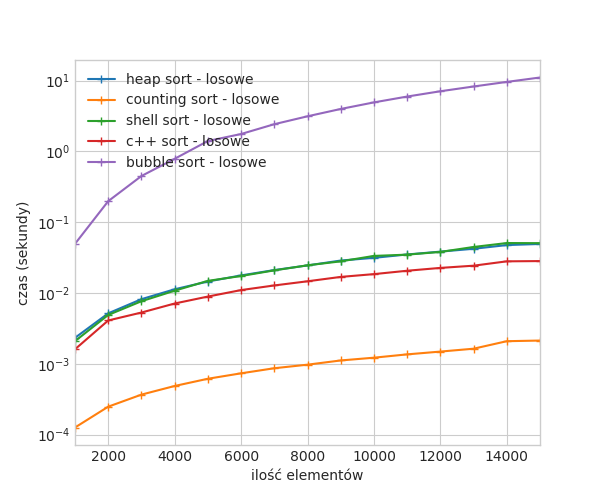
\includegraphics[width=\linewidth]{plots/los_bub_small_log.png}
	\caption{Czas sortowania danych losowych (małe dane, skala logarytmiczna) \label{losowe_male_log}}
\end{figure}

Pomiary czasowe na małym zbiorze losowych liczb, przedstawione na wykresie \ref{losowe_male}, weryfikują złożoność BS w przypadku średnim. Sortowanie $15\ 000$ losowych liczb zajmuje aż 11 sekund, podczas gdy inne algorytmy wykonują to zadanie w mniej niż 0,1 sekundy. Dla małych danych algorytmy HS i ShS mają podobny czas wykonywania. CS sortuje dane najszybciej. Te same wyniki są przedstawione w skali logarytmicznej na wykresie \ref{losowe_male_log}.



\subsection{Dane losowe duże}

Czasy sortowania dla większej ilości danych są przedstawione na wykresie \ref{losowe_duze}. Algorym BS został pominięty, ze względu na złożoność obliczeniową. CS nadal jest najszybszym z testowanych algorytmów, sortuje $1\ 000\ 000$ elementów w 0,1 sekundy. Jego czas wykonywania rośnie liniowo, zgodnie ze złożonością obliczeniową. HS i ShS sortują tą samą ilość elementów w odpowiednio 5 i 7 sekund.

\begin{figure}[h]
	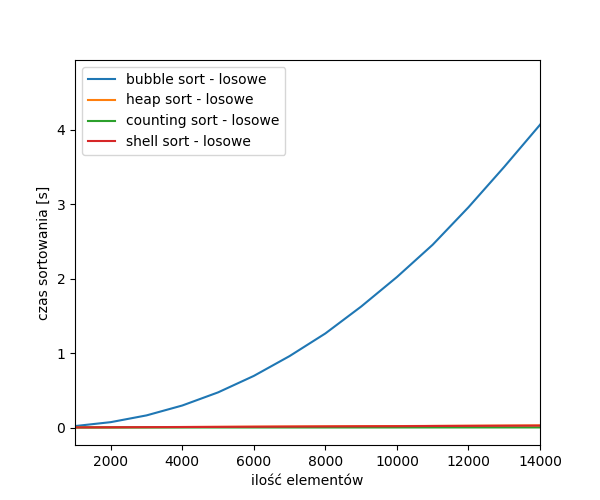
\includegraphics[width=\linewidth]{plots/los.png}
	\caption{Czas sortowania danych losowych (sortowanie bąbelkowe ukryte) \label{losowe_duze}}
\end{figure}



\subsection{Podsumowanie}

BS jest najmniej efektywnym algorytmem i nie powinno się go używać w żadnym przypadku. 

HS jest szybszy od ShS, w powyższych pomiarach. Wadą implementacji ShS, na której zostały wykonane pomiary, jest ciągłe dzielenie tablicy na dwie połowy. Istnieją jednak podziały, które pozwalają algorytmowi ShS uzyskać lepszą wydajność. HS i ShS mogą znaleźć zastosowanie w maszynach z ograniczoną liczbą pamięci (ponieważ sortują w miejscu), oraz gdy potrzebna jest korzystna złożoność obliczeniowa.

CS najlepiej radzi sobie z sortowaniem liczb. Algorytm ma zastosowanie gdy jest potrzeba bardzo szybkiego sortowania dużej ilości małych liczb (tu \emph{małą liczbą} było $10\ 000$). Przy większych lub bardzo oddalonych od siebie liczbach, CS zużywa więcej pamięci, co może być nieporządane. Implementacja może okazać się problematyczna, gdy dane do sortowania nie są liczbamy całkowitymi, lub nie są liczbami.



\section{Pomiary QS MS HS}

Następnie porównywane będą algorytmy quicksort QS, merge sort MS i heap sort HS.



\subsection{Dane losowe i stałe}

Dla losowych danych, QS ma najkrótszy czas sortowania. Sortuje on $1\ 000\ 000$ elementów w 1,5 sekundy. MS sortuje te same dane 2 razy wolniej, a HS 3 razy wolniej. 

Wszystkie algorytmy wykonują się w czasie o złożoności $O(n \log n)$.

Dane stałe najszybciej sortuje HS, $1\ 000\ 000$ elementów w 0,1 sekundy. QS sortuje tą samą ilość danych w 1 sekundę. MS wykonuje sortowanie 2 razy wolniej niż QS.
\begin{figure}[h]
	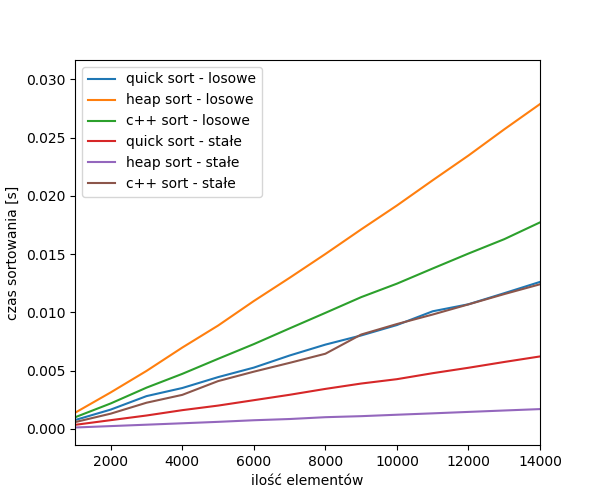
\includegraphics[width=\linewidth]{plots/ls.png}
	\caption{Czas sortowania danych losowych i stałych \label{losowe_stale_duze}}
\end{figure}



\subsection{Dane rosnące i malejące}

Czas sortowania danych rosnących i malejących jest podobny dla QS, MS i HS. QS sortuje najszybciej - $1\ 000\ 000$ elementów w 1 sekundę. MS wykonuje się 3,5 razy wolniej, a HS sortuje aż 5 razy wolniej niż QS. Wszystkie algorytmy sortują dane rosnące, malejące i losowe w podobnych czasach (wykresy \ref{losowe_stale_duze} i \ref{rosnace_malejace_duze}).

\begin{figure}[h!]
	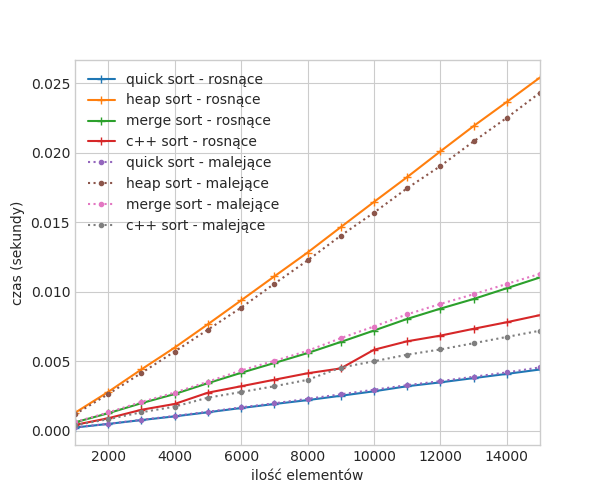
\includegraphics[width=\linewidth]{plots/rm.png}
	\caption{Czas sortowania danych rosnących i malejących \label{rosnace_malejace_duze}}
\end{figure}



\subsection{Dane a-kształtne i v-kształtne małe}

Dla danych a-kształtnych, zastosowana implementacja algorytmu, QS ma kwadratowy czas wykonywania; sortuje $15\ 000$ elementów w 2,5 sekund (dla porównania BS sortuje tyle samo elementów w 10 sekund). 

Ponieważ w tej implementacji, jako pivot wybierany jest zawsze środkowy element (a w danych a-kształtnych środkowy element jest największym elementem w tablicy), dane a-kształtne stanowią najgorszy przypadek dla QS.

Algorytmy MS i HS sortują dane a i v-kształtne o długości $15\ 000$ w mniej 0,1 sekundy, przy czym MS jest marginalnie szybszy od HS.

QS sortuje dane v-kształtne bez większego problemu, ale wolniej niż MS i HS - $15\ 000$ elementów w 0,1 sekundy.

Te same wyniki są przedstawione w skali logarytmicznej na wykresie \ref{av_ksztaltne_male_log}.

\begin{figure}[h!]
	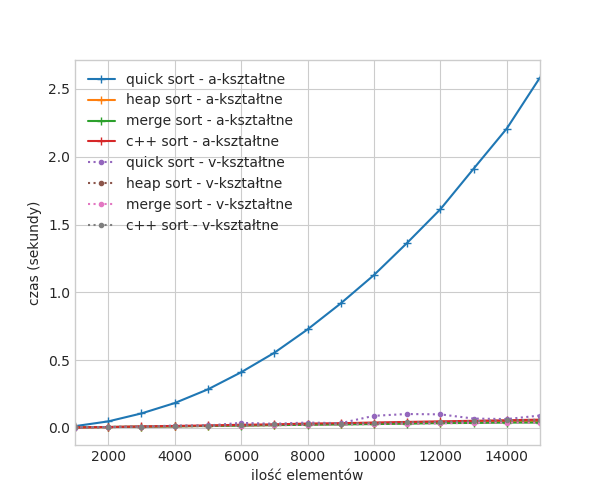
\includegraphics[width=\linewidth]{plots/av_small.png}
	\caption{Efektywność sortowania danych a i v-kształtnych (małe dane) \label{av_ksztaltne_male}}
\end{figure}

\begin{figure}[h!]
	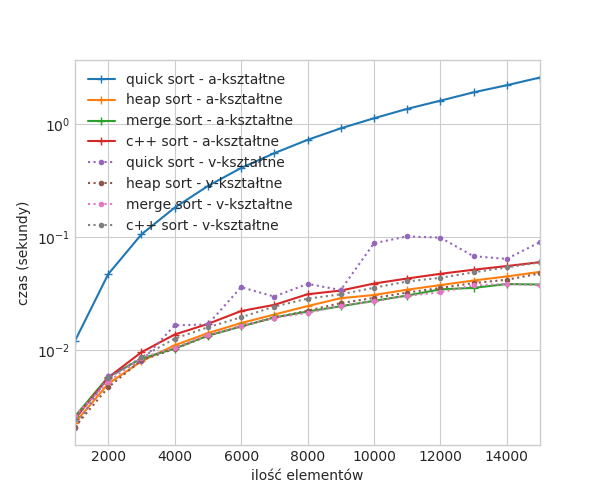
\includegraphics[width=\linewidth]{plots/av_small_log.png}
	\caption{Efektywność sortowania danych a i v-kształtnych (małe dane, skala logarytmiczna) \label{av_ksztaltne_male_log}}
\end{figure}



\subsection{Dane a-kształtne i v-kształtne duże}

\begin{figure}[h]
	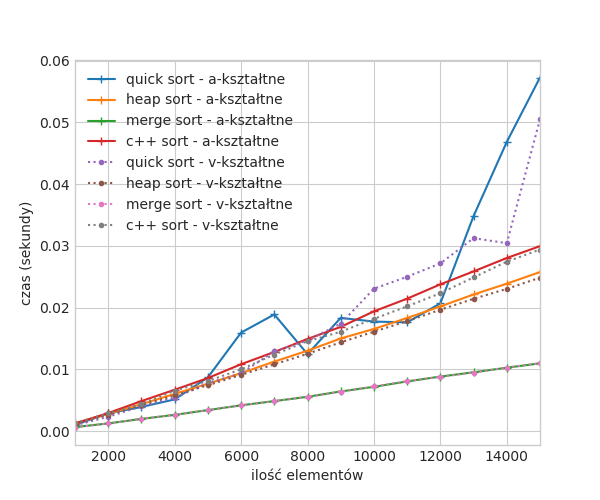
\includegraphics[width=\linewidth]{plots/av.png}
	\caption{Efektywność sortowania danych a i v-kształtnych (sortowanie szybkie ukryte) \label{av_ksztaltne_duze}}
\end{figure}

Czasy sortowania dla dużej ilości danych są przedstawione na wykresie \ref{av_ksztaltne_duze}. Algorym QS został pominięty, ze względu na złożoność obliczeniową, w tym zestawie danych.

Różnice pomiędzy MS i HS są wyraźnie widoczne przy sortowaniu $1\ 000\ 000$ elementów. MS sortuje te dane w 3,5 sekund, podczas gdy HS robi to w 4,5 sekund. 

\subsection{Podsumowanie}

Czasy wykonywania zarówno MS, jak i HS mają złożoność $O(n \log n)$. MS zużywa jednak dodatkowe ilości pamięci, co może być nieporządane na urządzeniach gdzie jest ona ograniczona.

W przypadku danych losowych, QS ma złożoność $O(n \log n)$ i jest szybszy od MS oraz HS, a przypadku danych stałych QS jest wolniejszy tylko od HS (także złożoność $O(n \log n)$). 

Algorytm nie radzi sobie z danymi a-kształtnymi i v-kształtnymi. Dla danych a-kształtnych ma złożoność $O(n^2)$. Jest to jednak specyficzne dla wybranego sposobu obierania pivota (zawsze środkowy).

Istnieją metody które zmniejszają szanse wybrania \emph{najgorszego} elementu jako pivota (najprostsza to wybieranie losowego elementu), w efekcie poprawiając wydajność czasową i pamięciową algorytmu.



\section{Quicksort i mediana}

Jeżeli podczas sortowania algorytmem QS jako pivot zostanie wybrana mediana zbioru, algorytm ma złożoność $O(n \log n)$ i czas wykonywania jest najkrótszy. Ilość rekurencyjnych wywołań jest mała. 

Podobnie dzieje się gdy w przypadku średnim, czyli kiedy wybór pivota jest losowy (lub sortowana tablica zawiera losowe elementy z równomiernym rozkładem prawdopodobieństwa).

Najgorszy przypadek następuje gdy jako pivot zostanie wybrany najmniejszy lub największy element z tablicy. Algorytm ma wtedy złożoność $O(n^2)$, a ilość rekurencyjnych wywołań jest bardzo duża. Przez to, podczas pomiarów dla danych a-kształtnych i v-kształtnych (dla ponad $50\ 000$ elementów) następowało przepełnienie stosu.



\subsection{Użycie mediany}

Dobrą metodą wyboru pivota jest wybieranie mediany z pierwszego, środkowego i ostatniego elementu tablicy jako pivot. Taki sposób wyboru pivota sprawia, że trudniej jest otrzymać najgorszy przypadek.

Zaletą tej metody jest to, że nie wymaga generowania losowych liczb, co może zajmować istotną ilość czasu, jeżeli losowość ma być wysokiej jakości, lub jeżeli nie mamy dostępu do dobrego generatora losowych liczb.



\end{document}

